% !TEX root =  ../main_manuscript.tex 
\section{Results}
The rate of reclassification at year five of follow-up was 35\% in PRIAS, and at most 50\% in the five validation GAP3 cohorts (Panel~B, Figure~\ref{fig:auc_beforecalib}). That is, many patients do not require any biopsy in the first five years of AS. 

In the fitted joint model, when patient age increased from 61 to 71 years (25-th to 75-th percentile), the adjusted hazard ratio of reclassification was 1.45~(95\%CI:~1.30--1.63). When fitted PSA value (log scale) increased from 2.36 to 3.07 (25-th to 75-th percentile), the adjusted hazard ratio was 0.99~(95\%CI:~0.89--1.11). When estimated instantaneous PSA (log scale) velocity increased from -0.09 to 0.31 (25-th to 75-th percentile), the adjusted hazard ratio was 2.47~(95\%CI:~1.93--2.99). Hence, instantaneous velocity of PSA was a stronger predictor of reclassification than PSA value. Detailed parameter estimates are in Supplementary~A.2.

The time-varying mean absolute prediction error, time-varying AUC, and calibration plot of our model in different cohorts are shown in Panel~B, Figure~8, Supplementary~B; Panel~A, Figure~\ref{fig:auc_beforecalib}; and Panel~B, Figure~\ref{fig:auc_beforecalib}, respectively. The AUC was moderate (0.55 to 0.75) in all cohorts. Mean absolute prediction error was large (0.3 to 0.45) in cohorts with rate of reclassification different from PRIAS, and moderate (0.1 to 0.3) otherwise. Our model required recalibration of baseline hazard of reclassification in all cohorts (Figure~6, Supplementary~B). Although, calibration was fine in Johns Hopkins cohort, whose rate of reclassification was similar to PRIAS (Panel~B, Figure~\ref{fig:auc_beforecalib}). The risk predictions from the recalibrated models were as good as risk predictions from joint models fitted separately to each cohort (Figure~7, Supplementary~B). Comprehensive validation results are in Supplementary~B.

\begin{figure}
\centerline{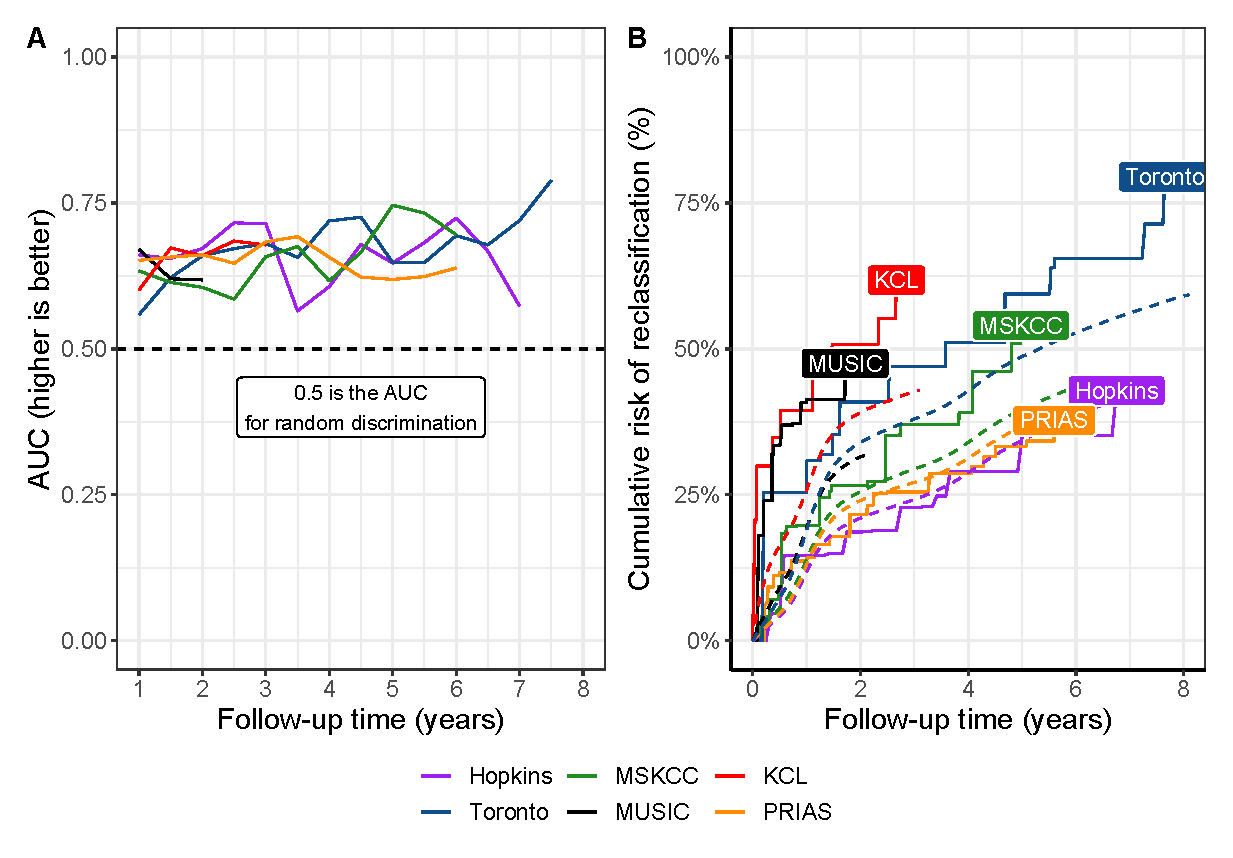
\includegraphics[width=\columnwidth]{images/auc_beforecalib.eps}}
\caption{\textbf{Model Validation Results}. \textbf{Panel~A}: time dependent area under the receiver operating characteristic curve or AUC (measure of discrimination). \textbf{Panel~B}: calibration-at-large~\citep{royston2013external,steyerberg2010assessing}, with solid lines depicting the non-parameteric estimate of the cumulative-risk of reclassification~\citep{turnbull1976empirical}, and dashed lines showing the average cumulative-risk of reclassification obtained using the joint model fitted to the PRIAS dataset. Full names of Cohorts are \textit{PRIAS}: Prostate Cancer International Active Surveillance, \textit{Toronto}: University of Toronto Active Surveillance, \textit{Hopkins}: Johns Hopkins Active Surveillance, \textit{MSKCC}: Memorial Sloan Kettering Cancer Center Active Surveillance, \textit{KCL}: King's College London Active Surveillance, \textit{MUSIC}: Michigan Urological Surgery Improvement Collaborative Active Surveillance.}
\label{fig:auc_beforecalib}
\end{figure}

Various personalized and fixed biopsy schedules for a demonstration patient in Figure~\ref{fig:demo_pat1} show that a personalized schedule based on 10\% risk threshold leads to one less biopsy than other schedules. At the same time, the corresponding time delay in detection of reclassification is expected to be only one month more than other schedules. A compulsory biopsy was scheduled at year six (maximum biopsy scheduling time in PRIAS, Supplementary~C) in all schedules for a meaningful comparison between them. Additional demonstrations are in Figure~9--11, Supplementary~C.